\documentclass[a4paper]{article}

%--- Load packages. 
\usepackage{amssymb}
\usepackage{amsmath}
\usepackage{framed}
\usepackage{textcomp}

% avoid ugly indentation of paragraphs
\usepackage{parskip}
\usepackage{graphicx}

% open sans font
\usepackage[default,osfigures,scale=0.95]{opensans}

% subfolder with the figures (within manuscript/)
\graphicspath{ {./figures/} }

% for author affiliations
\usepackage{authblk}

%allows inline citations
\usepackage[round]{natbib}
\bibliographystyle{plainnat}

% for degree symbol
\usepackage{gensymb}

% for line numbers
\usepackage{lineno}

% margin size
\usepackage{geometry}
\geometry{verbose,tmargin=3cm,bmargin=3cm,lmargin=3cm,rmargin=3cm}

% for bibtex
% \usepackage{authordate1-4}
% \bibliographystyle{authordate1}

%allows subscripts in text mode
\usepackage{fixltx2e}

%allows rotation of table??
\usepackage{rotating} 

%allows alignment of caption to the left
\usepackage{caption} 
\captionsetup[table]{singlelinecheck=false}

%allows not italic greek letters
\usepackage{textgreek}

\usepackage{Sweave}
\begin{document}
\Sconcordance{concordance:wtc1_paper.tex:wtc1_paper.Rnw:%
1 52 1 1 0 18 1 1 5 116 1}


\linenumbers

\title{Elevated atmospheric [CO\textsubscript{2}] and drought alters carbon allocation patterns in Eucalyptus saligna.}

\author[1,2]{Courtney E. Campany}
\author[1]{Craig D. Barton}
\author[1]{Remko A. Duursma}

\affil[1]{Hawkesbury Institute for the Environment, University of Western Sydney, Richmond, NSW 2753, Australia}
\affil[2]{Corresponding author (c.campany@uws.edu.au)}

\renewcommand\Authands{ and }
\maketitle

%--------------------------------------------------------------------------------------------%



%--------------------------------------------------------------------------------------------%
\section*{Abstract}

\section*{Introduction}

Carbon allocation is the proportional share of biomass production invested in the growth of foliage, fine roots and woody components per unit time (Mäkela 2012). Carbon allocation controls the flow of photosynthate between respiration and biomass production, and between short and long-lived above and belowground tissues (Epron et al. 2012). This distribution of new C among different pools and processes is an important factor in ecosystem biogeochemical and hydrological cycling (Warren et al. 2012), yet our knowledge of how environmental change impacts this distribution is incomplete. Understanding allocation is vital, as partitioning among plant organs and their feedback processes determines the growth rates of plant components (Friedlingstein et al. 1999, Lacointe 2000). 

Over-simplified models generally assume that a fixed fraction of assimilation is allocated to each organ (Franklin et al. 2012). Consequently, predictions of C partitioning among tree components under climate change are still unreliable (Palmroth et al. 2006), and the representation of C allocation is rudimentary compared to A in applied forest models (Friedlingstein et al. 1999, Franklin et al. 2012). For example, soil-vegetation-atmosphere transfer models are yet to incorporate a mechanistically based scheme for C allocation (Epron et al. 2012). The deficiency of large-scale models in their allocation components seems not to be due to a lack of empirical evidence, but rather to the difficulty in defining principles that are valid under a wide range of conditions (Franklin et al. 2012). Thus, accurate modeling of forest ecosystem metabolism and predictions of the effects of global change on C cycling is still hindered (Friedlingstein et al. 1999, Landsberg 2003, Litton et al. 2007, Epron et al. 2012). 

In a resource saturated environment a plant maximizes its growth rate by allocating new C to leaves to increase C acquisition (Monsi and Saeki 2005). However, environmental stresses such as water, nutrient and light availability may cause plants to invest in roots for belowground resources and stem elongation for increased light harvesting (Friedlingstein et al. 1999). These interactions are part of a dynamic system:  as the tree grows, or sink activities are altered, the fate of assimilate can shift through time. As a result, there is need to empirically measure patterns of tree C allocation under resource limitation in order to more accurately model forest C balance.

With rising atmospheric [CO\textsubscript{2}], forest C allocation has drawn particular interest due to its potential effect on C sequestration and the global C balance (Franklin et al. 2012). Increasing [CO\textsubscript{2}]  has been shown to stimulate net primary production and belowground C allocation, but the flux to belowground increased twice as much as aboveground productivity, as reviewed across four forested free-air CO\textsubscript{2} enrichment experiments (Palmroth et al. 2006). Additionally, understanding the impacts of global climate change on forests requires investigation of various global change factors to tease apart multifaceted relationships (Rustad 2008). In particular, as drought can limit plant productivity understanding potential interactions with the growth-stimulating effects of increasing [CO\textsubscript{2}]  requires further attention (Duursma et al. 2011). 

Allocation of C belowground remains one of the most difficult components of tree C budgets to calculate. In forest ecosystems, the flux of C belowground has been shown to be equal or greater than aboveground production (Law et al. 1999), yet the controls of this belowground flux are poorly understood (Raich and Nadelhoffer 1989, Giardina et al. 2005). As trees allocate such a large portion of production belowground, the difficulty in accurately measuring this allocation has limited our understanding of C cycling (Giardina and Ryan 2002). Consequently, modeling attempts to describe the response of belowground C allocation to global change often assume that responses of aboveground tissues represent those of belowground tissues (Giardina et al. 2005). These issues with both measuring and modeling tree C allocation elucidate a vital need to utilize a model experimental system which couples continuous measurements of assimilation and respiratory fluxes with the ability to track growth above and belowground.

The whole-tree chambers (WTC), located at the Hawkesbury Forest Experiment, were designed to allow continuous measurement of whole-tree net CO2 and water fluxes, allowing A, respiration and transpiration to be calculated using a mass balance approach (Medhurst et al. 2006, Barton et al. 2010). Generally, measuring canopy A is difficult as variation in photosynthetic capacity exists within the canopy in response to the environment, requiring leaf measurements and models to upscale to the canopy (Ryan et al. 2010). The WTC, however, can resolve net aboveground C gain (canopy A minus respiration of foliage and aboveground woody components, Figure 1.) at high temporal resolution, while controlling temperature and air humidity at ambient conditions. Belowground C flow, including root allocation, respiration and exudation, can then be estimated as the residual between net aboveground C gain and production of aboveground components. As a result, this experimental system provides a unique opportunity to validate models that scale from leaf gas exchange to the tree canopy with measurements of the response of whole-tree CO\textsubscript{2} fluxes and biomass production to global change manipulations (Barton et al. 2010).

The objective of this study is to determine the response of C allocation among foliage, aboveground woody components, and roots of a native Australian tree species, to changes in both atmospheric [COO\textsubscript{2}] and altered water availability. Specifically we test whether cumulative net aboveground C gain (Figure 1.) is correlate to whole tree biomass increment, as a function of tree size affected by drought and elevated COO\textsubscript{2}. Overall, the effects of drought and elevated COO\textsubscript{2} were expected to alter the fixed partitioning of C among biomass components from ambient conditions, which are commonly used in applied forest C models. Additionally, increased gross primary productivity in elevated [COO\textsubscript{2}] treatments will be the result of increased C allocation to roots, as similarly reported by Palmroth et al. (2006), and increases in C allocation to roots are also expected with drought treatments to reduce water limitation (Meier and Leuschner 2008), yet the interactive effects between the two treatments are still unknown.

\section*{Methods}

\subsection*{\textit{Whole tree chamber experimental design}}

From April 2007 Eucalyptus saligna Sm. seedlings were grown in 12 whole tree chambers (WTC) at the Hawkesbury Forest Experiment in Richmond, Australia. One seedling per WTC (10~m high) was grown for 2 years and chamber conditions tracked outside air temperature and humidity.  This multifactor experiment design included CO\textsubscript{2} × drought treatments with three replicates of in each of four treatments. Six chambers were kept at ambient atmospheric CO\textsubscript{2} concentrations (~380 ~ppm) and six were maintained at elevated levels of +240~ppm above ambient.  Through October 2008 all trees were watered with 10~mm of water every 3 days.  Next half of the chambers were subjected to drought treatments by completely withholding water, lasting through mid-February 2009. A final destructive harvest was completed in March 2009. Detailed descriptions of chamber design and operation are provided in Barton el al. (2010).

\subsection*{\textit{Tree chamber gas exchange}}
Floors installed above the soil surface permitted the chambers to functions as cuvettes and allowed for whole tree fluxes of CO\textsubscript{2} and water to be monitored once trees were ca.~3.5~m in height.  High resolution CO\textsubscript{2} flux data (ca.~14min intervals) were available for the final year of the experiment. For expression of chamber CO\textsubscript{2} fluxes on a canopy basis, through time, leaf area was estimated leaf counting in April 2008 and from the final harvest in March 2009. Canopy leaf area was interpolated through time height growth and litter fall rates, assuming that total cumulative leaf area followed and allometric relationship with tree height (Barton et al. 2010).

\subsection*{\textit{Allometric Tree Growth and Carbon Allocation}}
Tree height was measured bi-weekly. Stem diameters were recorded  monthly throughout the experimentmeasured at regular intervals along the main bole and split stems. Tree diameters at 65cm above the ground were used as the standard diameter because none of the trees had forks at this height. Canopy layers (5 in total) were set from the floor height and extended through the top of the canopy.  For the final harvest all plant mass is reported by canopy layer including leaf, twig, branch, and buds.  

\subsubsection*{\textit{Bole Carbon}}
Tree heights and diameters measured along the stem made throughout the duration of the HFE-I was used to determine the volume of the main stem from base to tip.  Individual volume units were constructed as concentric cylinders in between measurements of stem diameter.  This approach assumed stem taper was accounted in the differences between volume sizes across stem sections.  The last section which includes the top of the tree was calculated as a cone with a tip radius of .001~cm.  Tree heights and diameters measured along the stem made throughout the duration of the HFE-I was used to determine the volume of the main stem from base to tip.  Individual volume units were constructed as concentric cylinders in between measurements of stem diameter.  This approach assumed stem taper was accounted in the differences between volume sizes across stem sections.  The last section which includes the top of the tree was calculated as a cone with a tip radius of .001~cm.  The volume below the standard diameter (65~cm)  was calculated separately to interpolate taper into this section of the main stem.  Using the height of the tree and the diameter at 65cm the diameters at 30cm and at base were modelled by extending the length of the pre-existing cone. This resulted in two stem sections for the base of each tree with taper assumed as previously stated. All volume units were summed, including split stems, to calculate total tree volume.

During the final experimental harvest 1~cm stem sections were cut at regular intervals along the main stem to determine stem density.  Wood density was calculated as dry weight / fresh volume (kg m\textsuperscript{-3}), and was measured separately for bark and stem wood. Fresh volume (cm\textsuperscript{3}) was determined for each section through water displacement.  Diameters with and without bark were measured and then stem sections were oven dried to a constant mass.  For every tree bark and stem wood density were constructed for every stem section. 

Whole tree stem mass was calculated for approximately monthly for every tree coordinating with stem height and diameter measurements.  Stem wood mass and bark mass were calculated as volume multiplied by density for each volume unit, including a ratio parameter which corrects for the diameter proportion of bark:wood for each individual tree.  Bark mass and wood mass were then summed for all volume units for every tree.  Bole wood carbon was assumed to be 50$\%$ of mass, and this conversion was performed on all other subsequent plant dry mass components. Dry mass conversions by canopy layer were calculated oven drying sampled branches to a constant mass and water content was assumed to be constant within canopy layers.  


\subsubsection*{\textit{Branch and Twig Carbon}}

Branch mass (>1.0cm diameter) and twig mass (<1.0cm diameter) were estimated through time using separate equations. Branch diameter measurements were taken 5cm from their individual insertion points. During the final harvest 5 subset branches per canopy layer (n=5), covering a range of diameters, were sampled to obtain detailed measurements of architecture, allometry, and for dry mass determination. For each sampled branch the number of second order branches and composite twig mass was recorded. Basal area and length of each sample branch was determined and used to calculate the total branch volume. 5~cm was added back to each branch length in order to represent the entire branch volume. A volume shape factor, from Makela et al. (1995), was applied to each branch volume to designate each branch as an intermediate shape between a volumetric cone and a cylinder ($\phi\textsubscript{b}$, 0.75). Dry mass conversions by canopy layer were calculated oven drying sampled branches to a constant mass and water content was assumed to be constant within canopy layers. In order to estimate branch mass through time branch density ($\rho\textsubscript{b}$) was estimated for each canopy layer.  Due to the thin layer of bark in branches a seperate density parameter for bark was not created. Using the dry mass and volume of each sample branch, branch density was calculated as:

\begin{equation} \rho\textsubscript{b} = \frac{M\textsubscript{b}}{H\textsubscript{b}~\alpha~\phi\textsubscript{b}}
\label{eq:density}
\end{equation}

where M\textsubscript{b} is the dry mass, H\textsubscript{b} is the length, and $\alpha~\phi\textsubscript{b}$ is the basal area.

During the final year of the experiment branch diameter and length for each stem were collected across seven dates, including forked stems.  To obtain branch mass, volume was first calculated with all individual branches for each sample period as outlined above.  We assumed that branch density did not change through time and calculated branch mass at each time point~(i) as:

\begin{equation}  \text{M}^i_{b} = (\text{H}^i_{b}~\text{a}^i_{b}~\phi\textsubscript{b})~\rho\textsubscript{b}
\label{eq:branchmass}
\end{equation}

During the final harvest dry matter content of all twigs were recorded for each branch subset per canopy layer. Since allometric measurements were only recorded for branches, twig mass through time was estimated via the relationship between 

First, the number of second order branches was estimated for each branch according to branch length (r2 = 0.91, p < 0.001).  The dry mass of twigs was then estimated from the number of second order branches for each measured branch. Separate equations were developed for twig mass for branches with less than 20 (r2 = 0.61, p < 0.001) or greater than 20 second order branches (r2 = 0.72, p < 0.001).   Twig mass is reported as the sum of all modelled twigs for each tree through time.  

As twigs were not empirically measured through time (no allometry for branches less than 1cm) linear model equations were constructed from parameters within the detailed subset branch harvest. 

\subsubsection*{\textit{Leaf Carbon}}

Total leaf area and mass were measured for each of the five canopy layers for each WTC at the final harvest.  The relationship between cumulative tree leaf mass and leaf area was used to predict leaf mass through time for each WTC.  An additional leaf census was conducted in April 2008 and the development of leaf area through the final harvest was estimated based on height growth and litterfall. For April 2008, estimates of standing leaf area were obtained from total leaf counts for each tree, multiplied by tree-specific mean leaf size (based on a sub-sample). For March 2008, foliage biomass for each canopy layer was multiplied by canopy layer specific mean specific leaf area, and summed to obtain total standing leaf area.

For the model leaf growth was assumed to coincide with height growth, so that no leaf growth occurs when height growth has ceased.  We also make the assumption that total produced leaf area (i.e. standing leaf area plus that produced by litter fall) follows an allometric relationship with tree height such that:

\begin{equation}  \text{A}_{L,T} = \alpha~H\textsubscript{t}
\label{eq:leafarea}
\end{equation}

where $\text{A}_{L,T}$ is the total 'potential' leaf area, a and b are tree specific coefficinets and H is tree height~(m). Then standing leaf area at time t are obitained from tree height at time t and cumulative litterfall:

\begin{equation}  A\textsubscript{L} = \alpha~H(t)\textsuperscript{b} - \int_{t=0}^t~L(t)\textit{dt}
\label{eq:leafarea2}
\end{equation}

\section*{Methods}

Insert allometric relationships from methods here first

%--------------------------------------------------------------------------------------------%
\clearpage
\section*{Figures}

%wtc concept figure
\begin{figure}[h!]
    \centering
    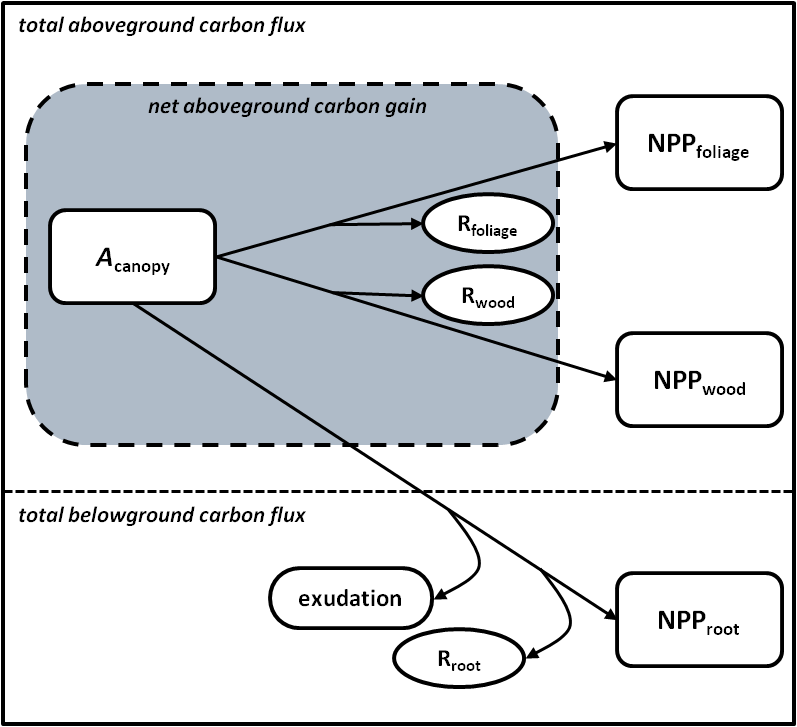
\includegraphics[width=0.99\textwidth]{wtc_concept.png}
    \caption{Conceptual diagram depicting the major components of C flow among plant components including; uptake via A, allocation to foliage, aboveground wood, roots, and losses through respiration and exudation.  Net aboveground C gain, shown in the shaded box, represents the flux of C measured within each WTC. }
    \label{fig:figure1}
\end{figure}

%fluxmass
\begin{figure}[h!]
    \centering
    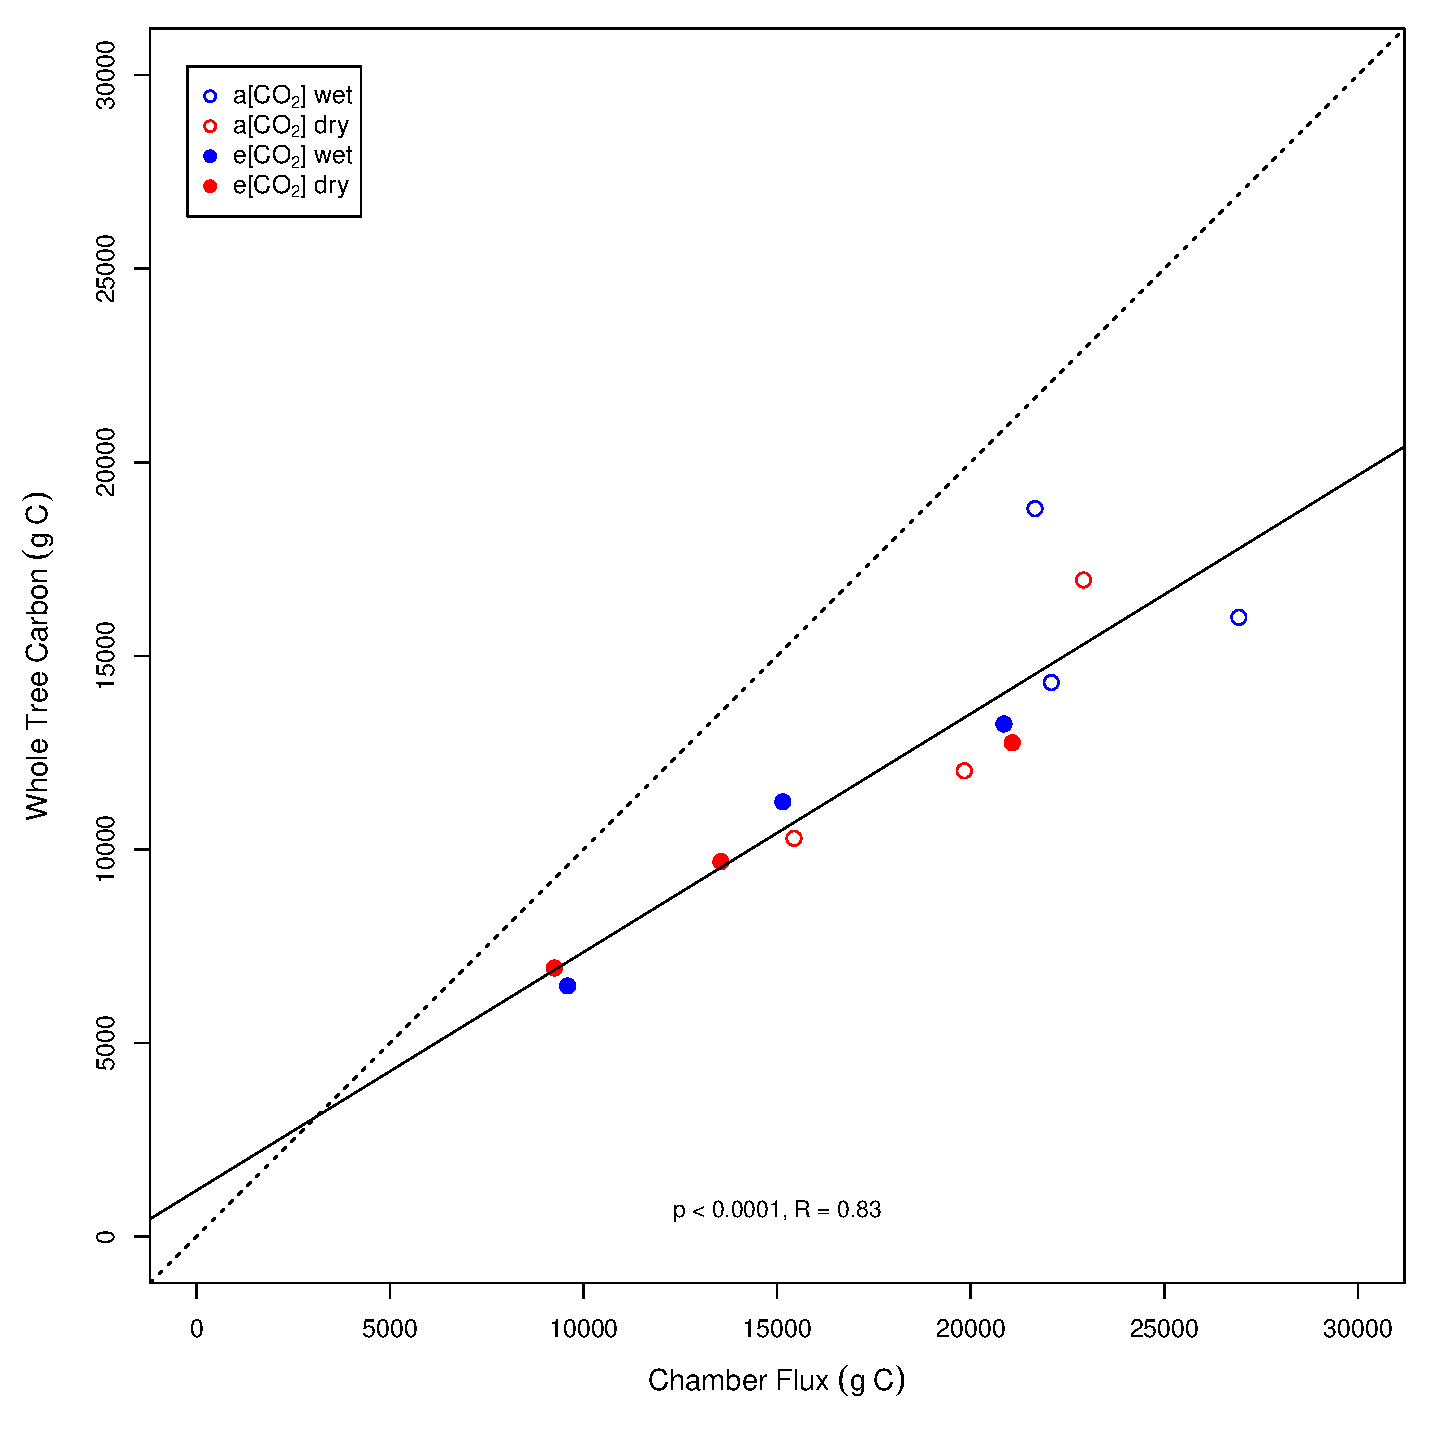
\includegraphics[width=0.99\textwidth]{WTCI_fluxmass.pdf}
    \caption{Harvested whole tree carbon mass as a function of cumulative whole tree chamber measured chamber C flux}
    \label{fig:figure2}
\end{figure}

\end{document}
